% %%%%%%%%%%%%%%%%%%%%%% file typeinst.tex %%%%%%%%%%%%%%%%%%%%%%%%%%%%%%  This
% is the LaTeX source for the instructions to authors using the LaTeX document
% class SVMultln with class option 'lnbip' for contributions to the Lecture
% Notes in Business Information Processing series. www.springer.com/series/7911
% Springer Heidelberg 2007/08/05  It may be used as a template for your own
% input - copy it to a new file with a new name and use it as the basis for your
% article. It contains a few tweaked sections to demonstrate features of the
% package, though.  If you have not much experiences with Springer LaTeX
% support, you should better use the special demonstration file ``lnbip.tex"
% included in the LaTeX package for LNBIP as template.
% %%%%%%%%%%%%%%%%%%%%%%%%%%%%%%%%%%%%%%%%%%%%%%%%%%%%%%%%%%%%%%%%%%%%%%%

\documentclass[lnbip]{svmultln}
\usepackage{makeidx}
\usepackage{amssymb}
\setcounter{tocdepth}{3}  
\usepackage{graphicx}
\usepackage{url}
\urldef{\mailsa}\path|sgossage@scs.carleton.ca|
\urldef{\mailRobert}\path|robert_biddle@carleton.ca|
\usepackage[pdfpagelabels,hypertexnames=false,breaklinks=true,bookmarksopen=true,bookmarksopenlevel=2]{hyperref}
\bibliographystyle{plain}


\begin{document}

\mainmatter

\title{CMAP: A Collaborative Multitouch Agile Planner based on Principles for Collaboration}


\titlerunning{CMAP}

\author{Stevenson Gossage and Robert Biddle}  
\authorrunning{Gossage and Biddle}
\institute{School of Computer Science, Carleton University, Ottawa, Canada\\
\mailsa, \mailRobert}

% \toctitle{TOC}
% \tocauthor{Gossage and Biddle}

\maketitle

\begin{abstract}

  Agile software development often involves two very simple but very
  effective supporting tools: the storycard and the cardwall.  This
  paper reports on our project to design a collaborative Agile planner
  based on principles for collabortion around interactive displays.
  The main goal of this project was to explore the use of multitouch
  enabled surfaces and how this technology could be leveraged to
  create a new level of usability in terms of group collaboration in
  Agile development. 

\keywords{Agile Software Development, User Stories,  Cardwalls, Multitouch Displays}
\end{abstract}
\section{Introduction}

Agile software development often involves two very simple but very
effective supporting tools: the storycard and the cardwall. These work
so well that we need to be cautious about applying any technology to
improve them. Recent advances in interactive display technology,
however, suggest that effective collaboration might now be supported
in a more lightweight way and in harmony with Agile
practices. Moreover, excellent work has been done on identifying
principles for collaborative behaviour around tables and displays.
This paper reports on our project to design a collaborative Agile
planner based on principles for collabortion around interactive
displays.

Both storycards and cardwalls work from the basis of stories
themselves, and as Cohn says, ``The technique of expressing
requirements as user stories is one of the most broadly applicable
techniques introduced by the Agile processes" \cite{StoriesRequ}.
Moreover, cardwalls act as what Cockburn call an {\em Information
  Radiator} \cite{InfoRad}, and help people maintain a situational
awareness of the state of the project, and also serve as place for
people to gather and discuss the project and state of the project and
quickly determine areas that need attention.  The role of physical
artefects, especially storycards and cardwalls, in Agile development
has been considered by Sharp, Robinson and Petre \cite{Sharp}, and they
show how there are both notational and social elements successfully at
work. Their results connect well with work in our own group, both on
social elements \cite{EWAgile} and on the nature of artefacts in
planning meetings \cite{JBAgile}. 

Large multitouch displays can be tables or walls. Their support for
handling multiple touchs allows recognition of multi-finger gestures,
such as pinching and twisting now commonplace on small-scale
multitouch devices such as the Apple iPhone.  But large-scale surfaces
also allow simultaneous use by more than one person, opening the door
to a new kind of support for collaborative applications. Principles for
the design of this kind of collaborative software have been identifies
by Scott, Grant, and Mandryk \cite{ScottGuidelines}, based on studies
of actual collaborative practices.

This paper describes the design of a software system, CMAP: A
Collaborative Multitouch Agile Planner. In this work, we began by
studying the earlier projects by Weber, Ghanam, Wang, Morgan and
Maurer at the University of Calgary \cite{Wang,Webber,DAP}. Their
projects used demonstrated the feasibility and utility of using
multitouch surfaces in support of Agile development. Our aim was to
explore some design alternatives based on consideration of the needs
for supporting flexible and lightweight collaboration. The Calgary
work used the Smart Technologies Smart Board and Smart Table and their
Microsoft Windows specific APIs. Our approach was to use open source
frameworks, in particular Python PyMT \cite{PyMt}, a framework
designed for the rapid development of multitouch UI prototypes and the
Community Core Vision (CCV) optical touch infrastructure, and our
software works on a range of hardware and operating systems.


\section{Background}

\subsection{Effectiveness of Agile Storycards and Storywalls}

Our work concerns on user stories, storycards, and cardwalls, and how
they are used by Agile teams. Of particular interest is their use by
the two most common lightweight Agile processes, Extreme Programming
\cite{XPvol} and Scrum \cite{Scrum}. Both of these methodologies take
an iterative approach where less focus is put on upfront analysis and
more on quick consistent deployment of quality working software.  We
intend our work to apply to both XP and Scrum, are we used terminology
from both.

Customers or product owners use storycards to record user stories
which describe features and requirements.  But the card is only a
token that represents a practice.  Jeffries describes the procedure as
the combination of the three C's, Card, Conversation and Confirmation
\cite{Jeffries}. The storycard is deliberately small, preventing
unnecessary verbose detail: Davies says ``The Card may be the most
visible manifestation of a user story, but it is not the most
important" \cite{PowerStories}.  She continues to explain that cards
``represent customer requirements rather than document them". This
emphasizes that the actual text on the card is simply a reminder or
placeholder; as Cohn says, ``the details are worked out in the
Conversation and recorded in the Confirmation"
\cite{UserStoriesApplied}. In the process of creating stories the
following should be considered, ``Words, especially when written, are
a very thin medium through which to express requirements for something
as complex as software. With their ability to be misinterpreted we
need to replace written words with frequent conversations between
developers, customers, and users. User stories provide us with a way
of having just enough written down that we don't forget and that we
can estimate and plan while also encouraging this time of
communication" \cite{UserStoriesApplied}.

The practice starts with the assignment of a story to a developer; as
Sharp et al. say: ``the physical possession of this card by a
developer is a warrant that secures the conversation (and the
confirmation process of them acceptance test) with a customer"
\cite{Sharp}. The subsequent communication between developer and
customer explores the details of the story and the confirmation,
should be mutually agreed upon, such that the story's completion is
well understood.  The cardwall is a tool where the storycards are
organized and displayed.  Typically new stories are placed in the
project backlog and remain their until they are scheduled for
development at which point they are removed from the backlog and
placed on the cardwall along with other stories also scheduled for
development. The grouping and or placement of stories on the cardwall
provides a visual cue as to the state of the stories. A natural
question might be to wonder how does this seemingly simply, low
technology solution helps software development teams to meet their
goals and deadlines while producing quality code? Often, it is the
human component that is the key to the success of the method. Any
software trying to replace a physical task must consider this issue in
depth and try and provide an environment, which supports and
encourages those same interactions, which bring success to the
physical task. 

Sharp et. al \cite{Sharp} strongly suggest that anyone considering
technology to support card and cardwall practices must take account of
the complex relationships that exist within this social system if they
wish to retain key properties of successful teams.  The following is a
summary of some of their key points.

While a general template for stories usually exists such that key
information is usually present like the {\sf As a <Role>}, {\sf I want
  <Description>}, and {\sf So that <Benefit>}, the process is
extremely flexible and we commonly find distinct notation across Agile
teams. At the same time, within any one team, people strictly adhere
to their agreed understanding of the notation and use of
cards. Everything on the card has meaning which is not necessarily
clear to an observer unfamiliar with the team specific notation.  The
location of, color, size of lettering and any annotations carry
significant meaning and thus provide a high level of abstraction. One
of the most compelling aspects of storycard is the flexibility it
affords teams to personalized notation in a manner that works best for
them. 

The use of the wall is also an extremely flexible procedure but, has
it's generalities in that, teams use walls for the duration of a
project and leave them on constant display somewhere they are easily
seen, usually, in a common space where stakeholders can quickly access
key factors like the progress of the project. The wall is generally
regarded as an ``Information Radiator" \cite{InfoRad} and helps
ensure the transparency of the project. Again, the wall is full of
meaning not obvious to an observer who lacks familiarity with Agile
methodologies or team-specific notation. Also again, the walls have
inconsistent structure across distinct teams, but are used in
extremely consistent manners within any one team.  Maybe more
important still are the social interactions involved in the whole
process; enabling teams to determine their best use of notation,
annotation and layout. These interactions reveal the importance and
meaning of the stories and thus drive their physical placement on the
wall, which, in turn radiates information about each story's progress.

\subsection{Multitouch Tool Support for Agile Development}

There are a limited number of software design tools developed to
harness the new possibilities in Human Computer Interaction afforded
by the current technology in multitouch enabled devices. Everyday more
devices are being produced at a reasonable cost with support for two
or more simultaneous touches; a critical feature for the development
of truly collaborative tools. The best example of similar software is
the Agile Planner for Digital Tabletop (APDT), \cite{Wang}.  APDT was
designed based on a prototype by Weber \cite{Webber} which was
intended for co-located collaboration on a single touch surface. APDT
chose to use this as a starting point but wanted to enhance it with
support for multitouch, the ability to interface with other Agile
planning tools and real world evaluation based on user studies;
observing traditional Agile planning meetings as well as observing
meetings conducted using DAP or Distributed AgilePlanner\cite{DAP} As
the name suggests DAP was designed to support distributed Agile teams
in the planning and maintenance of an Agile project through the use of
a digital whiteboard and storycards. DAP had been developed with a
traditional single user interface paradigm (one keyboard, one mouse)
such that users could collaborate from a distance but not so much in a
co-located environment. APDT also studied and drew from the literature
available on the use of multitouch tabletops in a group
collaboration. APDT was developed as a multitouch enabled tool,
specifically for two tables designed by Smart Technologies Ltd
(Smart), using Smart's proprietary SDK. The first table used DViT
(Digital Vision Touch) \cite{DVT} technology and had support for two
concurrent touches. The second table used FTIR (Frustrated Total
Internal Reflection) \cite{FTIR} technology and had support for 40
concurrent touches. The two touch capabilities of the DViT table
limited the user's ability to work concurrently while the small form
factor of the FTIR table meant that it was difficult to leverage its
support for 40 simultaneous touches. APDT was a highly functional full
featured tool, however, its dependence on the Smart SDK and therefore
on Smart's hardware helped us make a key design decision; we wanted
CMAP to be designed such that hardware and operating system
independence was a goal, as well as support for multiple concurrent
touches.

\subsection{Collaboration in Digital Workspaces}

Scott, Grant and Mandryk have considered studies of digital
workspaces, and identified guidelines for co-located collaborative
work on a large interactive displays \cite{ScottGuidelines}.  They
suggest there are eight key elements that must be addressed via the
physical hardware of the tabletop, via the software being used on the
tabletop or by a combination of the two. The following is a summary of
those key requirements and a brief description of each.


\begin{description}
\item[\bf Support interpersonal interaction:] The technology must support
  the mediation of the collaborative interaction and must not
  interfere with this interaction. Ideally it should be as natural to
  collaborate around a digital tabletop as it is to collaborate around
  a regular table.

\item[\bf Support for fluid Transitions between Activities:] Switching
  tasks during collaboration should be as seamless as possible. For
  example, if the activity needs to combine data entry and the ability
  to draw, then switching between these activities must be a natural
  process. This allows the focus to remain on communication. The use
  of multiple input mechanisms must be considered but, should be a
  feature that enhances the overall activity and not a hindrance for
  these transitions.

\item[\bf Support for Transitions between Personal and Group Work:] If the
  collaborative task involves a combination of both personal and group
  work, the system should try and capture this by providing a similar
  mechanism. The physical shape of the table might be a key factor for
  this point because the individuals must feel comfortable and their
  personal workspace must not feel cramped or invaded. One suggestion
  may be to support external devices or displays that could be used in
  conjunction with the digital tabletop. This approach may however,
  interfere with the fluid collaboration Scott suggests that this area
  needs more study.

\item[\bf Support Transitions between Tabletop Collaboration and External
  Work:] It should be easy to integrate previous work into the shared
  environment where it can viewed and manipulated as needed.

\item[\bf Support the use of Physical Objects:] The system should support
  both work and non-work related physical artifacts. For example,
  there should be no negative impact on the system if a non-work
  related object were placed on the table while the same action using
  a digital work related object might cause a communication link to be
  established, giving access to this work-related object.

\item[\bf Provide Shared Access to Physical and Digital Objects:] While
  collaborating around a traditional table, pointing and other
  gestures are usually easily interpreted by the group. On a digital
  surface this may not always be the case. A digital tabletop may
  provide several representations of the shared object (maybe one for
  each person) using gestures to try and point something out in this
  scenario could lead to confusion as users try to interpret how the
  gesture related to the object they are viewing. If however only one
  representation of the object is present, those same gestures may be
  a contributing factor to the overall understanding and group
  collaboration. The digital representation of shared objects is a key
  to the successfulness of the collaborative session. The designers
  must consider the potential physical locations of the participants
  as well as the possibility of obstruction by other users, objects or
  even gestures. Obvious examples of physical objects are digital
  artefacts like an IPad. A non-digital artefact might be the pieces
  or tokens of a board game implemented for the tabletop where users
  interact with the pieces in game-play.

\item[\bf Considerations for the Appropriate Arrangements of Users:] The
  system must be designed to accommodate sufficient personnel space to
  allow users to comfortably interact with each other without feeling
  cramped. Also, the intended audience is important because the
  physical difference between adults and children suggest that more
  children could comfortably interact around a table. Children also
  tend to want to be closer to their neighbours then most
  adults\cite{Aiello}. The system should also not be affected by
  participants repositioning themselves around the table. Virtual
  objects should be rotatable thus allowing equitable user interaction
  from any position.

\item[\bf Support Simultaneous User Actions:] This is an area where true
  hardware and software advancements have developed since the
  publication of Scott's paper in 2003. Most current tabletop
  implementations support both multiple input devices and concurrent
  user input.
\end{description}

\section{Design} Our primary strategy was to extend previous work on Agile tool
support by addressing key issues outlined by Scott et al. about group
collaboration around digital tabletops. Our second generation design also
attempted to address issues found by Sharp et al. about how the physical nature of storycards and cardwalls affect
their use and the social interaction of the process. Sharp and her colleagues
also makes it clear that software designed to digitise this process must carefully consider both the
notational and social aspects of these artefacts. 

During the implementation and testing of the initial system it became clear that
there was an unintended rigidity about the storycards and their use. This was 
later confirmed through discussion and feedback when the system was presented to
experienced Agile pratitioners. It was as a result of this feedback that a more 
flexible design was adopted and we tried to address some of the key points made 
by Sharp et al.

These issues gave birth to a new design and consequently a second version of
CMAP. In this section a discussion of the general design goals relevant to both
versions will be outlined, followed by the specific design of each version and 
the reasons for the change. Finally, an attempt will be made to outline specific
design elements that targeted particular aspects of the guidelines of Scott et
al.
\subsection{Basic Goals}
The basic goals of our design were:
\begin{itemize}
\item Support a digitised version of storycards and cardwall.
\item Support multiple concurrent inputs and users and multiple platforms.
\item Support gestures and the orientation independent use of the system.
\item Support for persistent data and shared.
\end{itemize}
To support these goals several design decisions were made including:
\begin{itemize}
  \item Use of PyMT and Python meant built in platform independence, multiple 
  concurrent user interaction and support for multiple inputs. PyMT allowed
  the use of gestures and rotatable widgets to deal with orientation issues.
  Furthermore, since both Python and PyMT are open source, we had the access and
  the freedom to change the code base when we found the need.
  \item The need to support persistent and shared data was achieved by using a  
  combination of open source projects including Git, GitHub and the Petaapan
  Google Application Server. Git took care of local and remote storage while the
  Google App Server took care of change notification through a publish subscribe
  mechanism and notification hook between it and the GitHub repository. 
\end{itemize}
The use of gestures was an important feature and a unique gesture was provided 
as a shortcut to all of the most important activities allowed by CMAP. Figure 
\ref{Gestures}, is a list of the custom gestures and a brief description. To 
create these gestures a tool had to be developed and this tool will be 
incorporated into the next version of the the software so that users can 
customize and create their own gestures mush like teams develop and use
distinct noations and layouts.
\begin{figure}[ht]
\begin{minipage}[b]{0.5\linewidth}
\centering
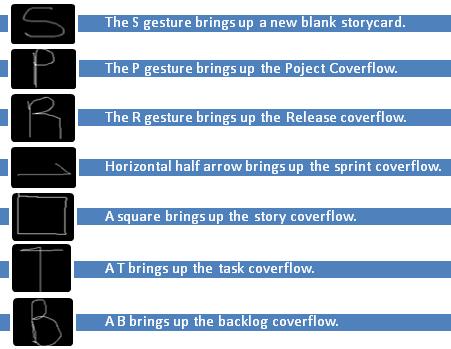
\includegraphics[width=5.5cm]{Gestures.png}
\caption[labelInTOC]{Custom Gestues}
\label{Gestures}
\end{minipage}
\hspace{0.5cm}
\begin{minipage}[b]{0.5\linewidth}
\centering
\includegraphics[width=5.5cm]{Coverflow2.png}
\caption[labelInTOC]{Coverflow, flipping the pages}
\label{Coverflow2}
\end{minipage}
\end{figure}



% \begin{figure}[htp]
% 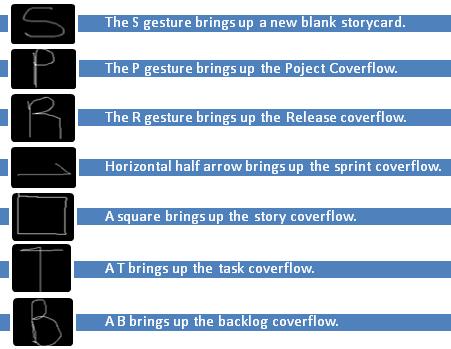
\includegraphics[width=10cm]{Gestures.png}
% \caption[labelInTOC]{Custom Gestues}
% \label{Gestures}
% \end{figure}
Throuout the design we made a number of key decisions related to the support of
Agile methodologies:
\begin{itemize}
  \item The wall traditionally gives structure to the stories and helps
  developers organise and manage their projects. To capture this functionality a
  hierarchical structure was created by organising artifacts in trees rooted in
  the project. In this way, artefacts could represent projects, releases,
  sprints, stories or tasks and the tree would be rooted in the project.
  \item The ability to group similar artefacts was considered important and the
  concept of a visual container was developed to be able to flip through 
  different artefacts of the same type. This gives the system the ability to see
  for example all the releases in a project or all the stories in a sprint (see 
  Figure \ref{Coverflow2} for an illustration).
\end{itemize}
% \begin{figure}[htp]
% \begin{center}
%   \includegraphics[width=10cm]{Coverflow1.png}
%   \caption[labelInTOC]{Coverflow, all pages on left}
%   \label{Coverflow1}
% \end{center}
% \end{figure}
% \begin{figure}[htp]
% \begin{center}
%   \includegraphics[width=6cm]{Coverflow2.png}
%   \caption[labelInTOC]{Coverflow, flipping through the pages}
%   \label{Coverflow2}
% \end{center}
% \end{figure}


% \begin{figure}[htp]
% \begin{center}
%   \includegraphics[width=10cm]{Coverflow3.png}
%   \caption[labelInTOC]{Coverflow, all pages on left}
%   \label{Coverflow3}
% \end{center}
% \end{figure}
\subsection{Version 1 Design Strategy}
Our first version took a structured approach to the storycard and cardwall. This
was an attempt to capture all the relevant data that seemed to be critical to the
Agile planning process. XML was used to define the data of the storycards and
other artefacts and the view was a form based widget with labels and text
fields.  Users could use traditional data entry via real or virtual keyboards.
In an attempt to limit the amount of information contained by an artefact, a
default minimal view was created which only allowed the entry of a name for the
artefact and a description. Figure \ref{fig:Minstory} shows the minimal artefact
view.
A second view was created for stories to allow the user to enter more 
information. This view was built so that the developer could, in conversation 
with the customer, elaborate on the information provided by the minimal view. 
Figure \ref{Fullstory} shows this more detailed view of a storycard. 

\begin{figure}[ht]
\begin{minipage}[b]{0.5\linewidth}
\centering
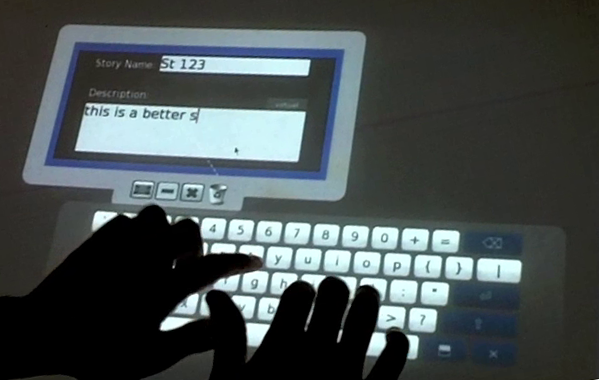
\includegraphics[width=5.5cm]{minstory.png}
\caption[labelInTOC]{Minimal Storycard View}
\vspace{-10pt}
\label{fig:Minstory}
\end{minipage}
\hspace{0.5cm}
\begin{minipage}[b]{0.5\linewidth}
\centering
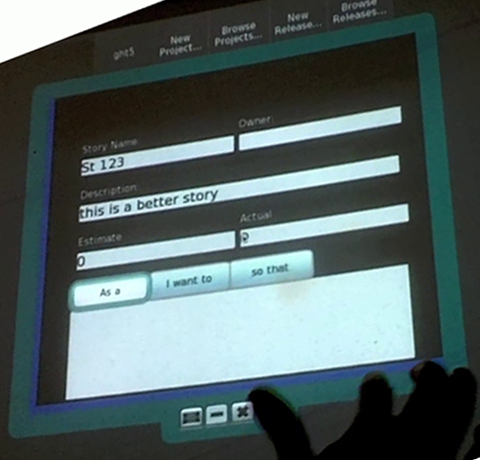
\includegraphics[width=5.5cm]{fullstory.png}
\caption[labelInTOC]{Full Storycard View}
\vspace{-10pt}
\label{Fullstory}
\end{minipage}
\end{figure}
% \begin{figure}[htp]
% \begin{center}
% \begin{tabular}{cc}
%   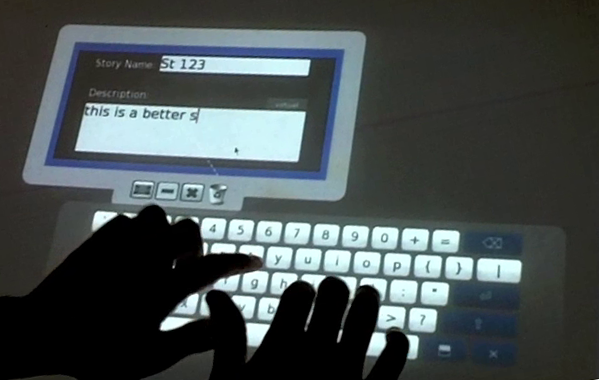
\includegraphics[width=5.5cm]{minstory.png}&
% %   \caption[labelInTOC]{Structured Minimal Storycard View}
% %   \label{Minstory}
%   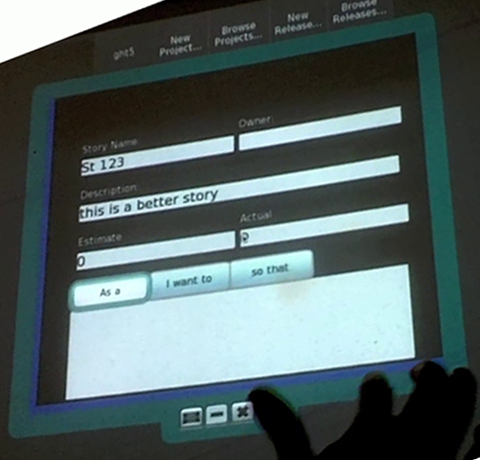
\includegraphics[width=5.5cm]{fullstory.png}
% %   \caption[labelInTOC]{Structured Full Storycard View}
% %   \label{Fullstory}
% \end{tabular}
% \end{center}
% \end{figure}
% \begin{figure}[htp]
% \begin{center}
%   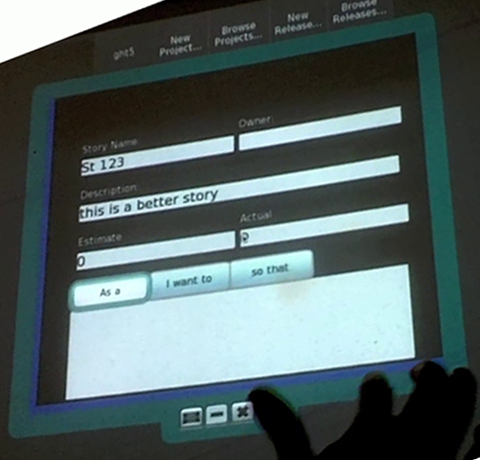
\includegraphics[width=6cm]{fullstory.png}
%   \caption[labelInTOC]{Structured Full Storycard View}
%   \label{Fullstory}
% \end{center}
% \end{figure}
% \end{tabular}

This structured approach seemed like a good way to capture the data and have it
in a format that could easily be stored, shared and adapted to allow it to 
interface with other software tools like task management systems. This approach 
could give developers access to the stories directly from their IDE.
\subsection{Version 1 Walkthrough}
The user starts by creating a project. Once created the next step is to create one or more releases, then one or more
sprints, then one or more stories and finally if they choose to they could
create one or more tasks. The only flexibility in this process is the ability to
create stories at any point which are then placed into the backlog. Coverflow
widgets were designed to hold artefacts of the same type. These containers are
initially empty, except for the ability to create a new artefact of that type.
So, to create a project the user could draw a {\sf P} gesture to bring up the
project container. From the container, clicking on the New Project button would
bring up a new empty project artefact. This process makes the newly created project
active such that a new release would automatically become a child of this
project. This introduces the concept of the {\em current} artefact which is
intended to control the hierarchical structure of the artefacts. For each artefact type,
there could be a current artefact of that type. This allows the system to create
the parent-child relationships of the artefacts automatically. For example once
a project is created, it becomes active and will automatically become the parent
of all newly created artefacts, if however, a second new project is created, it
would then become the new current project and subsequent artefacts would become
the children of this new project. To bring up the releases container one would
use the capital {\sf R} gesture. Again there is a button to create a new release. In
a similar fashion the user can use the gestures outlined in Figure
\ref{Gestures} to bring up the other containers, and create artefacts of those
types. The capital {\sf S} gesture was reserved as a shortcut to skip the story
container and create a new story directly. As each artefact is created it
becomes active and the creation of new artefacts either become siblings or
children of the current artefact. However, if creating siblings these new
artefacts then become the current artefact of this type. For example a user
could go through the process up to creating a sprint, at which point the
creation of many stories may be desirable, and as each one is created, it
becomes current, allowing the optional creation of tasks for that story.

\subsection{Version 2 Design Strategy}
In the course of development the direction that was originally taken came into
question for various reasons. Two important questions arose as a result of
demonstration and consultations with expert practitioners and researchers. The
first was a question of flexibility of user interaction with the system and the second was
how might the rigidity of the design adversely affect or interfere with the
human aspects of the process. In an attempt to address these concerns the
original structured implementation was redesigned. The form-based approach to
the stories and other artefacts was replaced by a more flexible drawing 
widget which was called a {\em scribble} widget. The intent was to allow users
to enter anything they wanted on the cards, imposing no rules; much like the
flexibility afforded them when using physical cards. The scribble widget allowed
the user to scribble notes on the card anywhere, as well as providing a
mechanism to do text entry via virtual or real keyboards (see Figure \ref{Scribblecard}
for the illustration). The text entered had the added flexibility of being able
to be repositioned anywhere on the card. There was also the ability to erase all
or parts of the information including text. The XML representation of the data
was only slightly modified to allow for these changes. Two new fields were added
to accommodate the new information, including a list of points and text widgets,
the colours, size and positions also needed to be stored. This allowed the data
to be picked up by remote applications and the cards could be re-drawn as
identical copies.

% \begin{wrapfigure}[6]{r}[\columnwidth+\columnsep]{9cm}
% \centering
% \includegraphics[width=0.3\textwidth]{figure.jpg}
% \caption{My figure.}
% \label{fig:myfig}
% \end{wrapfigure}

\begin{figure}%{r}{12cm}
\begin{center}
  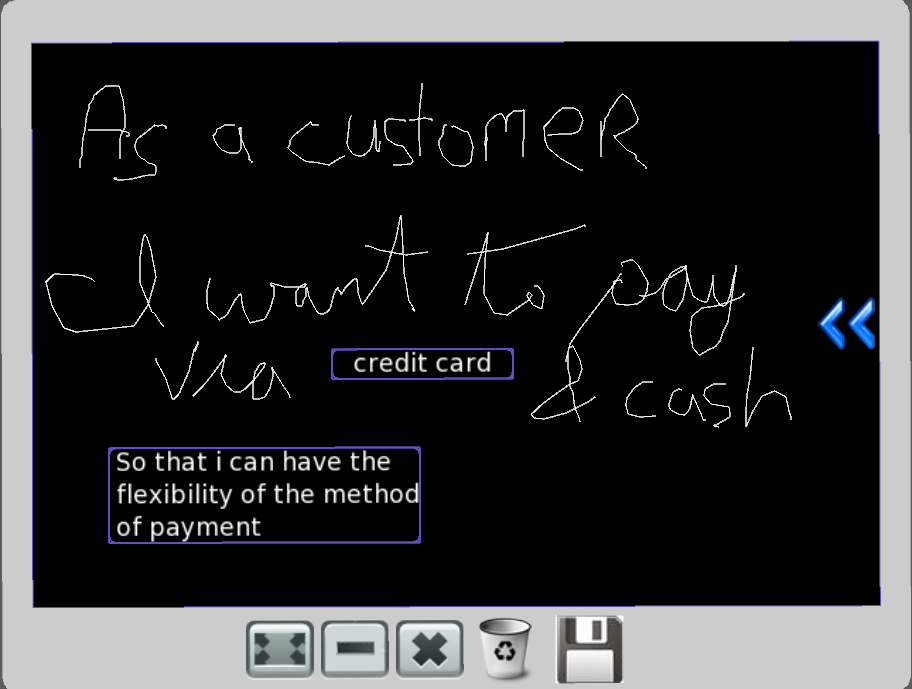
\includegraphics[width=7cm]{ScribbleStoryCard.png}
  \caption[labelInTOC]{Scribble Storycard}
  \label{Scribblecard}
  \vspace{-10pt}
\end{center}
\end{figure}

\subsection{Compliance with guidlines by Scott et al.} 
\subsubsection{Support Interpersonal Interactions}
Collaboration is a communicative process driven by human
interactions and this is supported by CMAP in that the software makes no
deliberate attempts to interfere with this driving force. The real success of
this claim needs to be explored through ecologically valid user studies. In 
future implementations an attempt to capture this interaction will be made by
integrating the capability to record the planning session either as a whole or any individual part of the planning meeting
including voice recording controls which can be enabled or disabled on key
artefacts like individual storycards as well as in the shared workspace (the
cardwall).

\subsubsection{Support for Fluid Transitions between Activities}
The original CMAP design had no handwriting capabilities and therefore had no
real transitions between different types of user input; although it may have
been fluid it was too rigid for a truly collaborative application. The revised
version allows the user to seamlessly transition between data entry via keyboard
or handwriting. CMAP has built-in support for multiple user input devices via
the PyMT framework. This allows the application to support multiple users
interacting with the system concurrently. For example multiple users could all
be creating and working on different stories at the same time. Multiple users
could technically also edit a story at the same time but, just as with the paper
storycard, the size of these widgets may limit the usefulness of this process.
The PyMT framework also has built-in support for other input devices such as
stylus or even the Nintendo Wii Remote.

\subsubsection{Support for Transitions between Personal and Group Work}
Transitions between personal and group work will be supported in future versions
of this application. In particular the future work already being considered and
planned for to support these types of transitions are:

\begin{itemize}
  \item Create a personal space work widget which will be a modified coverflow. 
   The traditional coverflow widget is static and displays its child artefacts
  as pages in a book which you can flip through page by page. The modified
  coverflow widget will allow the user to transform the widget (scale, rotate
  and move). Each user will have their own coverflow to use as a personal work
  area in which they can create and manage their artefacts in their own personal
  space. The widget must be capable of enabling or disabling a shared view of
  all or part of their widget. By default the widget will be private with the
  user being able to share any part as necessary. The widget will support the
  seamless transition from the current artefact to any adjacent artefact plus
  the ability to quickly jump to an artefact that is physically separated by
  many artefacts. The primary method of sharing artefacts contained in a user�s
  personal coverflow will be to drag the artefact to the shared workspace which
  essentially creates a copy of the artefact in the public domain where it can
  be manipulated by all users. The coverflow will have a smaller scaled view to
  support easier interaction and placement of the contained artefacts into the
  shared workspace as well as the ability to maximize any one artefact in the
  user�s personal workspace.

  \item The primary goal of this shared workspace will be to simulate a story  
  wall where stories are placed and sorted into releases, sprints, etc. Most
  importantly the shared workspace is intended to enhance the collaborative
  experience and facilitate discussion which is a critical component, necessary
  to ensure the success of any Agile based design meeting.
\end{itemize}
\subsubsection{Support Transitions between Tabletop Collaboration and External
Work} 
Future versions of this software will support a variety of external work inputs 
and outputs:
\begin{itemize}
  \item Allow handheld devices to interact and exchange data with the
  application (from cell phones to laptops).
  \item Allow the application to seamlessly allow data import and export to and
  from external applications. This should include other Agile development tools,
  bug trackers, schedulers and task management software. Direct integration into
  the developers IDEs, starting with Eclipse, using Mylyn as a task management
  system is an objective.

  \item The largest benefit of this software may in fact lie in its ability to  
  inter-operate between devices and an ideal setup might in fact be a digital
  table top for group collaboration combined with a wall mounted surface to
  truly give the look and feel of the traditional paper based Agile design
  process.
\end{itemize}
\subsubsection{Support the use of Physical Objects}
Currently the PyMT Framework supports the use of stylus pens, Wii Remotes and
as stated in the previous point future versions will support the use of other
digital artefacts. Secondary physical objects are to some degree
supported by the hardware in that many tabletops for example provide a border
where items like drinks or notepads can be placed without interfering with the
application.

\subsubsection{Provide Shared Access to Physical and Digital Objects}
Most of the widgets in the application are rotatable which gives users the
opportunity to use them in any appropriate orientation. When artefacts are in
the shared workspace gestures like pointing should be easily understood and thus
should contribute to the collaborative process. Careful consideration and
further study may reveal to what extend the application needs to support other
types of physical objects.

\subsubsection{Considerations for the Appropriate Arrangements of Users}
The physical size of the table and for future versions, the wall should dictate
the number of users that could comfortably interact with the system. The future
ability to use handheld devices should allow for more simultaneous user
interactions and therefore allow for more participants especially when
interacting around the wall. The only parts of the program that that cannot be
rotated are the menus.  Using these menus may be sensitive to the orientation of
the users. These menus are however, optional since gestures are available to
replace the menu items functionality and the gestures have no orientation. The
rest of the widget, as stated previously, can be rotated to suit the needs of
the users. For future versions where the personal workspace is implemented there
will need to be careful consideration as to how the system reacts when people
physically change their positions around the workspace. One simple solution
might be similar to what might happen in a real meeting. For example, in a
traditional pen and paper style meeting the task at hand requires that you
change your position for whatever reason and you forget to bring all your
personal stuff it may be reasonable to simply ask someone to pass your things to
you; since all the artefacts are draggable this could easily be accomplished by
CMAP.

\subsubsection{Support Simultaneous User Actions}
The support for simultaneous user actions is limited only by the hardware since
the PyMT framework gives the application support for any number simultaneous
user actions. This support is of utmost importance to the success of any
software designed to support co-located group collaboration.

\subsection{Distributed Agile Teams}
Although explicit support for distributed Agile teams was out of scope, it is
supported in a limited fashion. This support includes the ability to work using
the application in different locations and when data is saved it will be
available to all applications that have registers with the Google app server. While not real time collaboration it does give distributed
teams the ability to share their artefacts. Figure \ref{ClientServer} is shows the relationships between the StoryApp controller and
the local GIT repository, the GitHub server and the Google App Server.
\begin{figure}[htp]
\begin{center}
  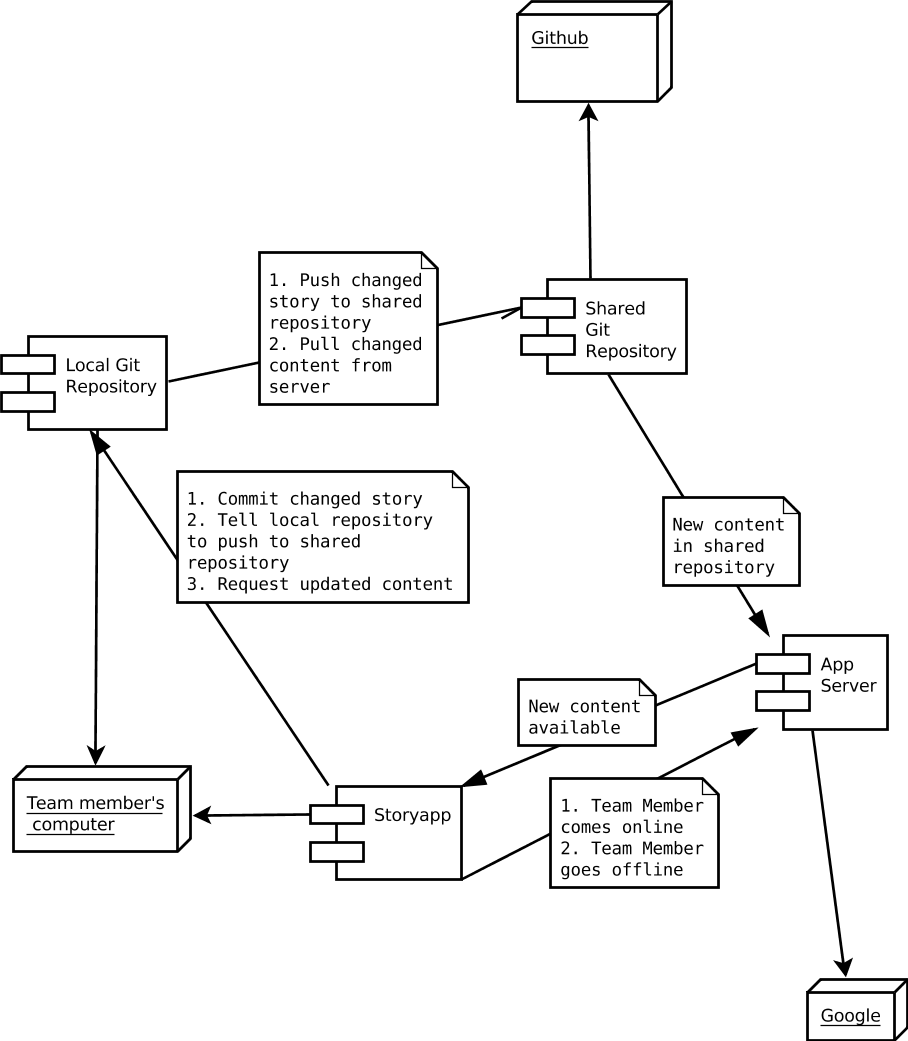
\includegraphics[width=8cm]{ClientServerDiagram.png}
  \caption[labelInTOC]{Relationships between Git, GitHub and Google App Server}
  \label{ClientServer}
\end{center}
\end{figure}

\section{Discussion}
Many enhancements could be made to the system such as the following list of
features that will be added to CMAP in subsequent versions:
\begin{itemize}
  \item The system must have an out of the box default behaviour that is
   intuitive and useful but it also needs to provide teams with the flexibility
   of adapting it to fit their particular process. Any method particular to a
   team should be configurable and supported by CMAP. This may include the
   team�s use of color, symbols and notation. We need the ability for
   the user to define all of this notation such that for example a scribble or
   text of a certain color might signify to the system that what is being
   written is a {\sf benefit} or a {\sf As a}, {\sf Want to} or {\sf So that} type of
   field. Likewise a certain symbol placed on the card could signify that this artefact
   is in progress, assigned etc. This flexibility is important but at the same
   time it should be up to the user to decide if they want to use this
   capability and not force it on the users. That being said, we must remember
   that the more the system understands the meaning of the content the more
   useful the digitization of the system becomes, especially in terms of
   overhead, duplication of work and interfacing to existing tools.
  \item The storycards themselves should have a way to be flipped such that the
   back of the card is usable and maybe a way to simultaneously view both back
   and front of any one artefact. 
  \item Default templates to allow users to base their artefacts on a predefined
   structure. These templates should be fully customizable. Different templates 
   based on difference in common uses of the cards. 
  \item Each card needs the ability to record audio (via the display device
  itself) to try and capture the social interaction and intent of each story. 
  \item Similarly, the whiteboard or wall should have its own flexible recording
   capabilities to capture the interaction during the sorting, prioritization
   and scheduling of the stories. 
  \item Ideally a collaborative group area, like a digital table, combined
   with an information radiator, like a digital wallboard, as well as the
   ability to toss stories onto the wall or table from other portable devices
   or remote computers.
  \item The recognition of handwriting is critical in order to interface and
   exchange data with other tools.
  \item Size matters; the cards must not be re-sizable other then maybe the
   ability to see both sides simultaneously as previously mentioned. The
   physical size ensures a true communicative process and dialog between
   developers and customers (although we still want to be able rotate and
  obviously move them).
\end{itemize} 
\subsection{The PyMT Multitouch Framework} 
We used the PyMT framework\cite{PyMt} for many reasons including its support
for multiple concurrent input devices, its rich library of widgets and support 
for gestures. Since it is an open source framework, any extensions or 
modifications needed could be easily applied. It clearly provided many highly 
useful features but, most importantly, because it is platform and operating 
system independent, it gave us the ability to run the app on a variety of 
hardware available to us in the lab. We had two, 2-touch LCD monitors (a 22-inch
Dell and a 24-inch Acer) hooked up to our deveopment systems and found that 
ability to test as we coded was invaluable. We also of utmost importance for
our application to run on out Smart Technologies Ltd. FTIR table and on our
custom built DI (Diffuse Illumination \cite{DI}) table. 


\section{Conclusion}
Multitouch enabled
hardware and software provides a new interface that is very well suited for
group collaboration. In particular, it gives developers of collaborative design
software, the tools needed to address many of points outline the paper Scott et
al. paper on the guidelines for group collaboration around a digital tabletop.
CMAP provides an open source platform independent framework that can be used to develop and test
further concepts in co-located and distributed collaboration. These concepts can
be tested on any number of multitouch enabled hardware devices. This flexibility
is important for future study aimed at establishing guidelines for the best
combination of size, resolution, number of concurrent touch inputs and shape of
future multitouch devices for the express purpose of group collaboration in a
design setting. The novel use of the distributed code repository may also be
considered important; it demonstrated a clean reusable solution to the difficult
problem of sharing versioned data and the possibility to remotely collaborate
using the shared distributed repository.

A number of important lessons were
learned during the development and use of the two versions of CMAP. The most
important is to consider the relations between the physical actions being
performed and the cognitive processes that facilitate the activity. A user that
picks up a storycard from a backlog pile and places it on a pile for a
particular sprint is hopefully thinking ``I am scheduling this story into that
sprint" rather than ``this is how I move this card to that pile". It is important
that the physical gestures not interfere with the flow of thought. Far too often
in computer based systems this is not the case and the necessity to perform
several computer interactions to execute a seemingly simple operation interrupts
the train of thought.

CMAP can be used as a starting point for future study. Of particular interest
would be to conduct user studies to observe its usefulness in a real world
project development process in both collocated and distributed teams. Further
development of the application could then be explored, implementing the results
of those findings combined with the continued development of the system with the
addition of the features outlined in the Implementation section. Further
exploration of improvements needed for the real-time collaboration in
distributed teams is critical for the system to be successfully integrated as a
widespread tool in industry. Furthermore, there needs to be more exploration
with respect to the potential use of 3D graphics in conjunction with multitouch.
PyMT is fully OpenGL compatible and will permit the exploration of rich
alternatives to existing means of interaction.

As software engineers and developers we are constantly presented with the
opportunity of creating software intended to replace activities traditionally
performed using pen and paper. Although our ability to design and implement
these systems is improving, we still tend to fall short more often than not.
``Research has shown that the versatility of paper contributes to its persistent
use in many work environments, even along-side computers meant to replace
it" \cite{ScottGuidelines}. Key factors that
contribute to this failure have been outlined in this paper. Most important is
the flexibility of the system, and the human factors that make the activity a
success. The digitization of tasks must consider the communication, mediation
and human interactions that are inherent in the tasks, and must be designed in a
way to encourage or enhance these interactions (or at the very least, not
interfere with them).

\bibliography{XP_2011_bib}

\end{document}


